% \textbf{\underline{OZ 2 - Magnetische velden - Oefening 3:}}
% \vspace{0.5cm}

% Een cirkelvormige lus met straal $ R $ draagt een stroom $ I $. De lus wordt in een magnetisch veld geplaatst waarvan de rechte veldlijnen lijken te divergeren vanuit een punt dat in het midden onder de lus op een afstand $ d $ ligt. Bepaal de kracht op de lus.

% \begin{description}[labelwidth=1.5cm, leftmargin=!]
%     \item[Geg. :]   $ R $; $ I $; $ B $; $ d $;
%         \begin{figure}[H]
%             \centering
%             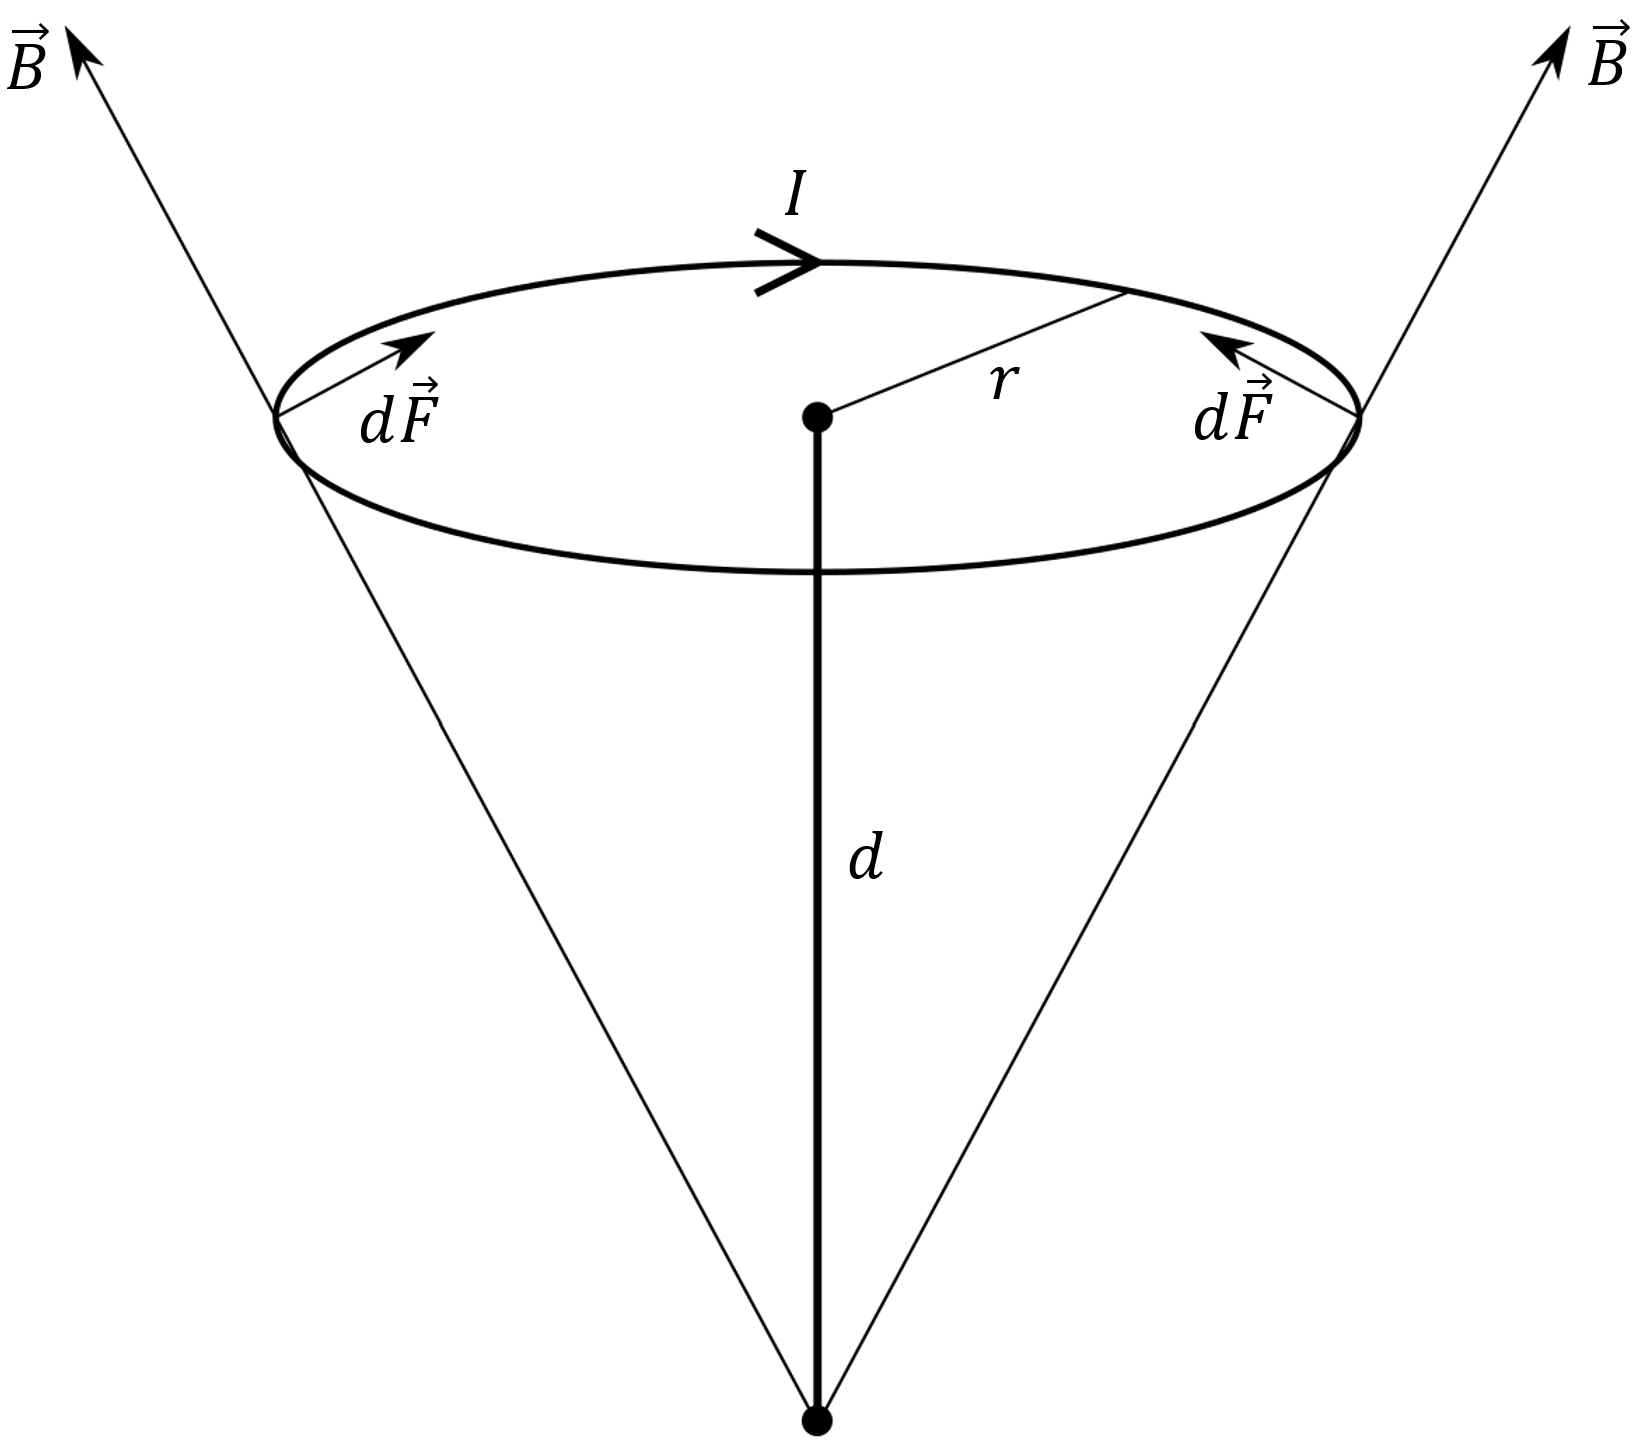
\includegraphics[width=8cm]{oz02/resources/oef-3-schets.png}
    
%             \textbf{Schets 2.2}
%         \end{figure}
%     \item[Gevr. :]  $ \vec{F} $;
%     \item[Opl. :]   $ d\vec{F} = I d\vec{s} \times \vec{B} $
                    
%                     \hspace{-0.57 cm} $ \Leftrightarrow 
%                     dF = I ds B $ \hspace{2.5cm} $ (\theta = 90^{\circ} \Rightarrow \sin{\theta} = 1) $
                    
%                     De $ x $-componenten van $ dF $ heffen elkaar op omdat ze symmetrisch naar het middelpunt van de lus wijzen, deze mogen we dus negeren.
                    
%                     $ dF_y = dF \cdot \dfrac{R}{\sqrt{R^2 + d^2}} 
%                     = \dfrac{I R B}{\sqrt{R^2 + d^2}} ds $
                    
%                     $ s $ loopt van 0 tot $ 2 \pi R$ (Omtrek cirkel)
                    
%                     $ F = \int_{0}^{2 \pi R}{\dfrac{I R B}{\sqrt{R^2 + d^2}} ds} 
%                     = \left[ \dfrac{I R B}{\sqrt{R^2 + d^2}} s \right]_0^{2 \pi R} = 0 - \dfrac{2 \pi I R^2 B}{\sqrt{R^2 + d^2}} = - \dfrac{2 \pi I R^2 B}{\sqrt{R^2 + d^2}} $
                    
%                     Omdat we weten dat $ F $ geen $ x $-component heeft kunnen we de kracht ook schrijven als
                    
%                     $ \vec{F} = \dfrac{2 \pi I R^2 B}{\sqrt{R^2 + d^2}} (-\hat{j})$
% \end{description}

% \vspace{1cm}